\section{Preprocessing}
In this step, our goal is to build an offline data structure according to Probase's taxonomy, so that the runtime system (search process) can quickly return queries that contain concepts found in user query. In brief, the preprocessing step is to generate a model file of inverted index that can provide an index from Probase concept to queries in query log.

The preprocessing step is performed in two steps - conceptualization and aggregation. First, we \textit{conceptualize} each instances found in each historical query from query log to some certain Probase concepts, resulting in an intermediate file with index from queries to concepts in the form of "\textit{query-id $\to$ concept-ids}". In the second step, we reorganize the intermediate file into an inverted index format from concept to queries in the form of \textit{"concept-id $\to$ query-ids"}.

\subsection{Conceptualization Step}
In this step, we aim at conceptualizing instances in historical queries. In order to achieve that, first, we parse the query into a sequence of \textit{keywords} and Probase instances. Then, we conceptualize each instance into Probase concepts using the \textit{isA} relationship information from Probase. We define a \textit{keyword} as a single word, which is neither an instance nor a concept in Probase.

The parsing process uses a similar algorithm with Parser, i.e. maximum-match algorithm (Algorithm \ref{alg:parse}), 
which will be presented later. For example, if we find a phrase 'president obama' and assuming that 'president', 
'obama', and 'president obama' are all valid instances in Probase. The algorithm will take the longest possible 
one - 'president obama' - as the recognized instance.

For conceptualizing instances, we use typicality information of each instance, which is a part of Probase. Each 
instance $i$ has a list of pairs ($c$, $t$), where $c$ denotes a Probase concept in which this instance can be 
conceptualized into and $t$ denotes a \textit{typicality} value of how likely the instance $i$ relate to the 
concept $c$.

At the end of this step, the system will produce an intermediate file for later step. Each line starts with a 
\textit{query-id} followed by \textit{instance-id} for instances found in the query, \textit{concept-id} of 
the super concept of the instance and the typicality value. The Fig. \ref{fig:conceptualization} shows how the 
intermediate file is organized.

\begin{figure}[h]
\centering
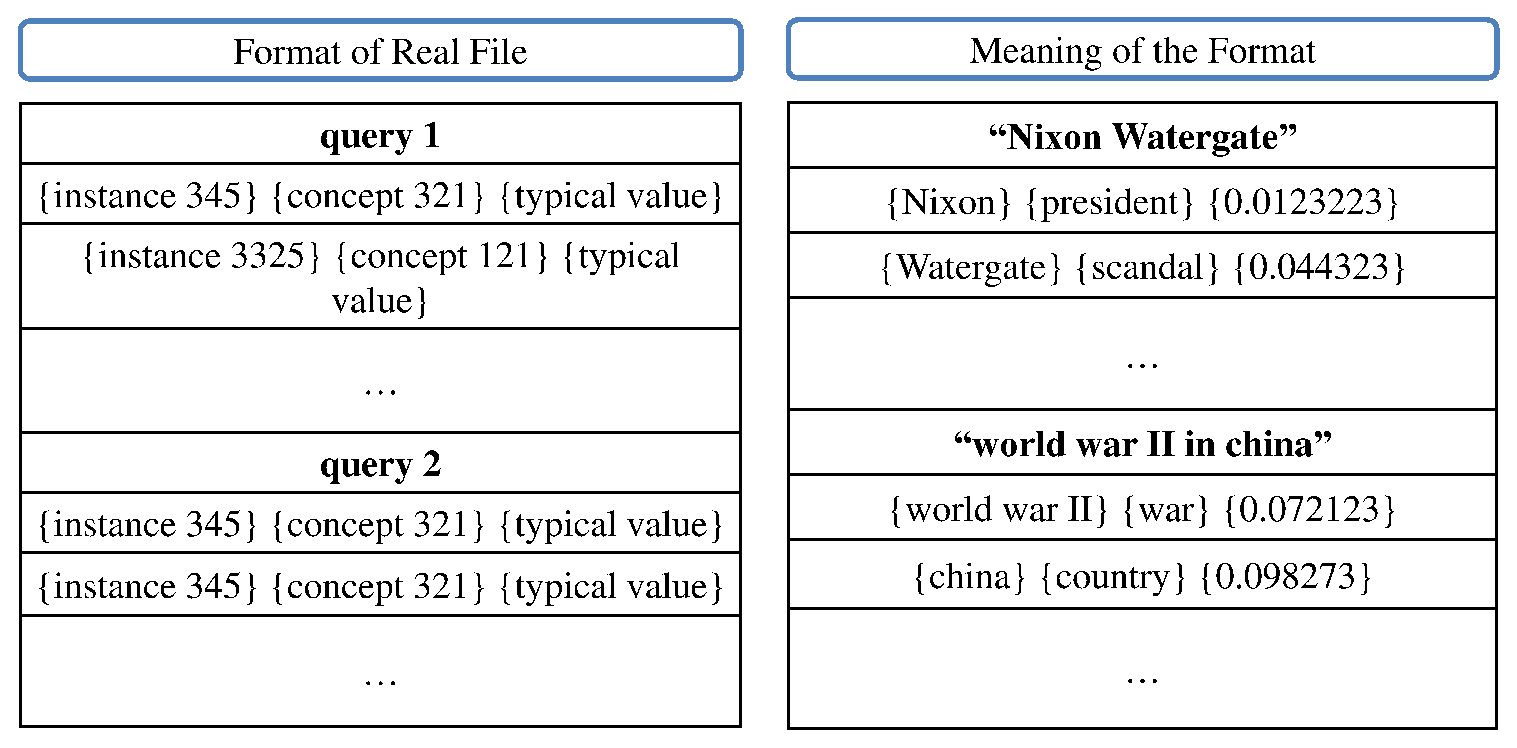
\includegraphics[scale=0.3]{images/conceptualization}
\caption{Format of Conceptualization Model File}
\label{fig:conceptualization}
\end{figure} 

\subsection{Aggregation Step}
We convert the format of the intermediate file produced in conceptualization step and produce the final aggregation 
file. The intermediate file is organized by unit of query, while the aggregation file is an inverted index organized 
by unit of concepts. The Fig. \ref{fig:aggregation} illustrates the format of the aggregation file.

\begin{figure}[h]
\centering
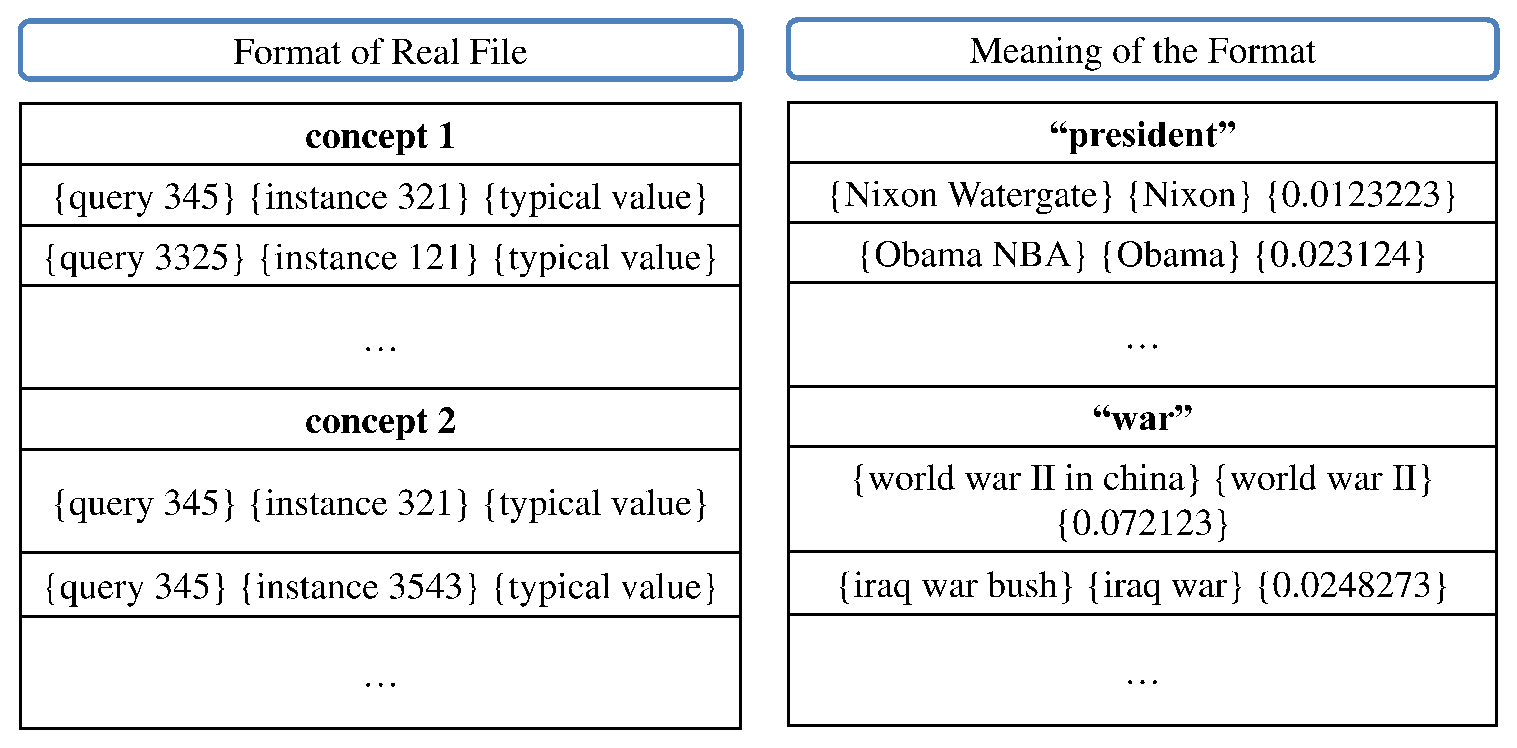
\includegraphics[scale=0.3]{images/aggregation}
\caption{Format of Aggregation Model File}
\label{fig:aggregation}
\end{figure} 

\subsection{Space Complexity Analysis}
\label{sec:spaceAnalysis}
In order to make a clear description, we define the following notations:

\begin{itemize}
  \item $n$: total number of historical queries in query log.
  \item $I_{hq}$: average number of Probase instances in each historical query.
  \item $C_I$: average number of Probase concepts, that a Probase instance can be conceptualized to.
\end{itemize}

Using the above notations, we can see that in average each historical query will be stored $I_{hq} \times C_I$ times in the aggregation file. Because there are $n$ queries in search log, the overall space complexity of aggregation file will be $O(I_{hq} \times C_I \times n)$. In this case, if we consider $I_{hq}$ and $C_I$ as constant, the overall space complexity of preprocessing will be $O(n)$, linear to the size of the query log.
